% File generated by nTex - Java Application for fast notes in LaTeX
% by Jarda Vitku

\documentclass[journal,onecolumn]{IEEEtrancz}
% zvolte kodovani
\usepackage[utf8]{inputenc} % linux/unix
%\usepackage[latin2]{inputenc}
%\usepackage[cp1250]{inputenc} % Windows
\usepackage[czech]{babel}
\usepackage{graphicx}
\usepackage{makeidx}         % allows index generation
\usepackage[bookmarks=false, colorlinks=false, unicode]{hyperref}

%\usepackage{enumitem}
%\setlistdepth{9}

\begin{document}

\title{Name of the document}
\author{Name of Author}

\maketitle

\begin{abstract}
	Abstract in one Line..
\end{abstract}

\IEEEpeerreviewmaketitle



\section{Section}
Some normal text..

\begin{itemize}
	\item itemized text
	\item Some text in \textbf{bold} and \textit{italics}.
	\begin{itemize}
		\item higher level..

\end{itemize}
\end{itemize}
\subsection{Some subsection here}

\begin{itemize}
	\item Here is an example of some citation: \cite{kniha}.
		\vspace{3mm}
		\vspace{3mm}
	\item This item is separated by means of several enters from the above one
	\item Here we add some figure Obr.\ref{a} 

	\begin{figure}[ht]
		\centering
			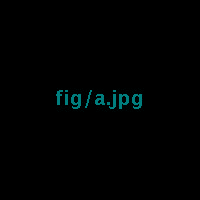
\includegraphics[width=2.0cm]{fig/a.jpg}
		\caption{Description of figure}
		\label{a}
	\end{figure}

	\item Here is another reference to already placed figure Obr.\ref{a} 
	\begin{itemize}
		\item Note that you don't have to specify width or description to the figure Obr.\ref{b}.

		\begin{figure}[ht]
			\centering
				
\includegraphics[width=6.5cm]{fig/b.jpg}
			\caption{ something..}
			\label{b}
		\end{figure}

		\item Type of figure is determined automatically,currently supported types are:
		\begin{itemize}
			\item eps
			\item png
			\item jpg


\end{itemize}
	\end{itemize}
\end{itemize}
\begin{literatura}{1}

\bibitem{kniha} 
Allman J.: \emph{Evolving Brains}, Scientific American Library Paperback, 2000.
\end{literatura}

\end{document}
